\section{Results}\label{sec:results}
The learning curves in Figure~\ref{fig:dshift_offline_normal} show the
$Q$-values evolution for the standard agents as a result of offline
training, while the ones in Figure~\ref{fig:dshift_offline_ensemble}
show the same metric for their respective ensemble version. Every
proposed offline agent learns to solve both classic control
environments, and the reward curves are presented in
Appendix~\ref{sec:appendix}.
% NOTE maybe this sentence is not even necessary
The reward signals for the \texttt{CartPole-v1} environment are
noisier compared to the ones for \texttt{Acrobot-v1}; this is in line
with the performance of the online behavioral DQN agent
$\pi_{\textrm{DQN}}$, which also produced unstable learning curves on
the problem.

\subsection{Offline bootstrapping error in the DQV family}
\begin{figure}[!tbp]
  \centering
  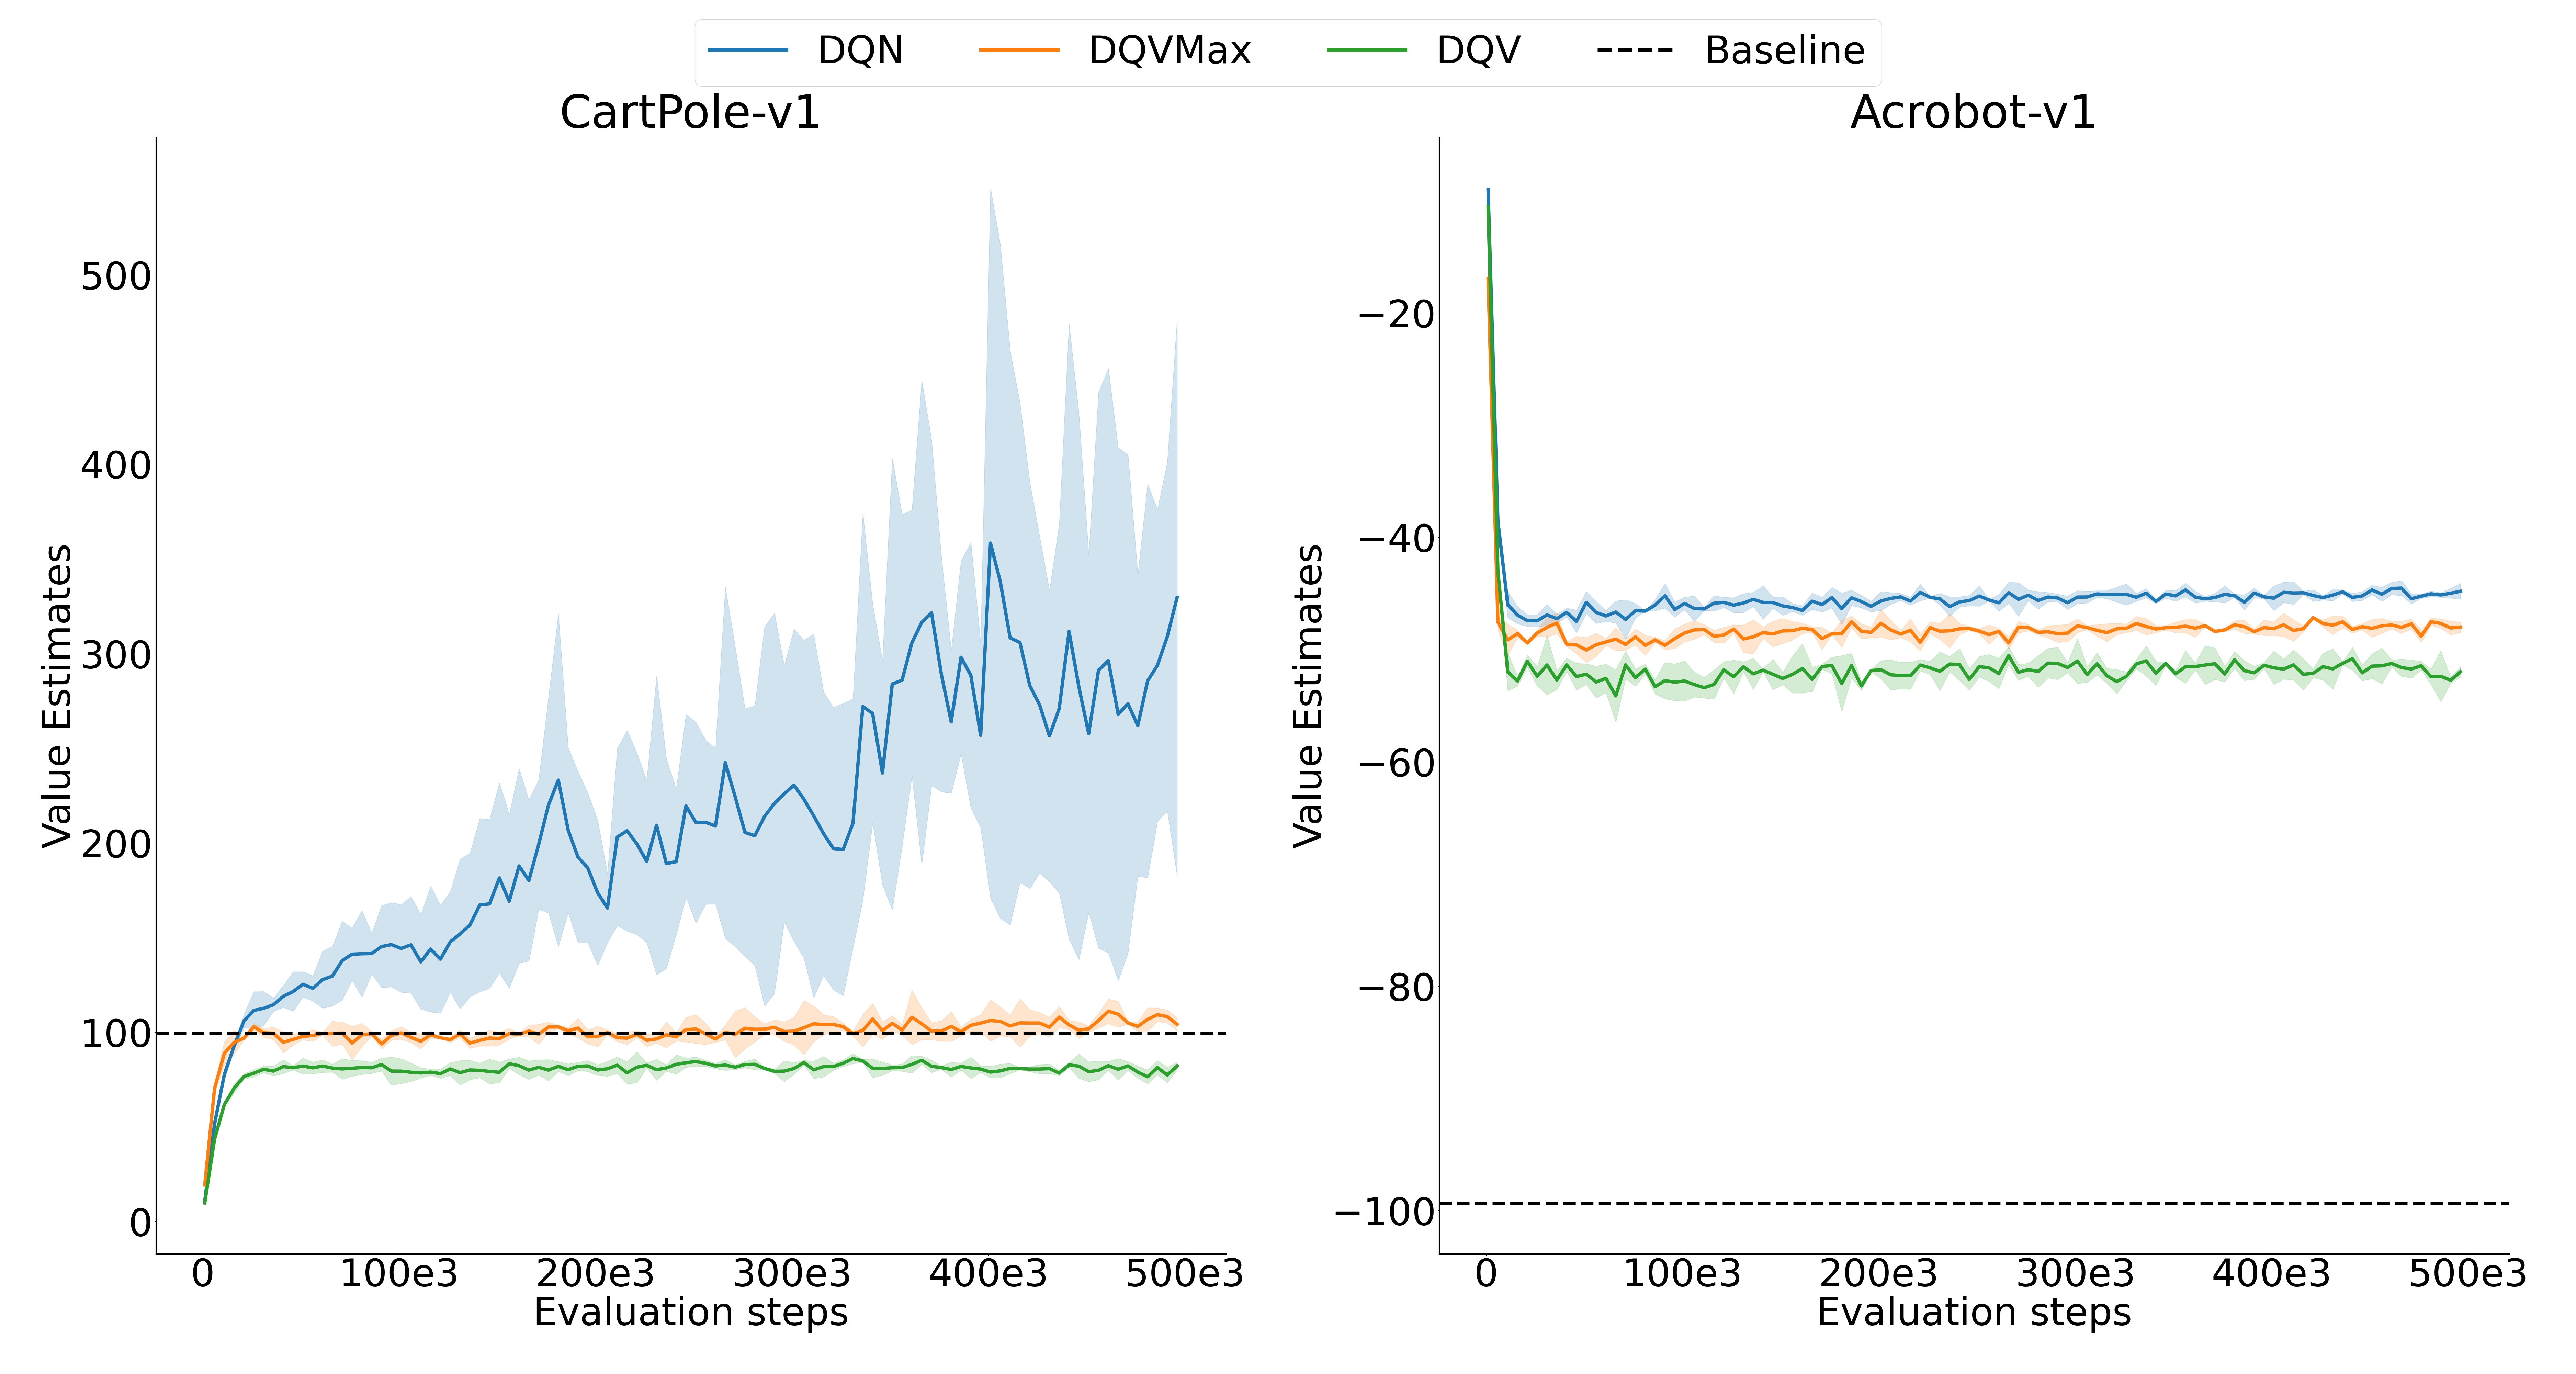
\includegraphics[width=.5\textwidth]{img/dshift_plots_qv.png}
  \caption{The $Q$-value estimates of offline DQN, DQV and DQV-Max at
    evaluation time. The shaded areas are $\pm 1$ standard deviation
    from the mean of 3 different
    simulations.}\label{fig:dshift_offline_normal}
\end{figure}
% Q estimates discussion for:
% DQN offline
As seen in~\ref{fig:dshift_offline_normal}, the experiments confirmed
previous findings for Q-learning-based gents run offline on continuous
domain problems \citep{pmlr-v97-fujimoto19a,kumar2019stabilizing}: the
$Q$ function incurs in a heavy overestimation bias produced by
bootstrapping errors. This is most evident on the \texttt{CartPole-v1}
environment, where DQN's $Q$-value estimates quickly escalate above
the true value. Since the offline agent has no access to ground truth
values due to lack of exploration, it cannot adjust the $Q$ function
estimates during training and the whole estimation process
diverges. Offline DQN suffers overestimation on the
\texttt{Acrobot-v1} problem too, but no divergence in $Q$ estimates is
observed here; this is likely because the behavioral data for this
environment are less noisy compared to those of \texttt{CartPole-v1}.

% DQV offline
Among the studied algorithms, offline DQV is the most robust one to
the bootstrapping error. On the \texttt{CartPole-v1} environment it is
almost able to correctly estimate the true value of $s_0$ for each
episode, never incurring in overoptimistic estimates. However, on the
\texttt{Acrobot-v1} problem, offline DQV still suffers from stable
overestimation, despite coming closest to the true value of $s_0$.
DQV avoids the bootstrapping error because it is an \textit{on-policy}
algorithm. Although theoretically it should not be able to learn in
the offline setting, its strong
performance compared to the other agents is probably due to efficient
usage of the large offline dataset, which enables it to learn on-policy
discovering effective behaviors in the data. Moreover, DQV forms its
TD-target using only the state-value function $V$, therefore it cannot
possibly base predictions on those very out-of-distribution actions
which are responsible for bootstrapping errors.

% DQV-Max offline
Offline DQV-Max is also more resilient to the bootstrapping error than
offline DQN.\ On the \texttt{CartPole-v1} environment, it estimates
the true value for $s_0$ nearly perfectly, showing no detrimental
effects due to misaligned bootstrap estimates. As it is the case for
offline DQV and DQN, it still overestimates the real $Q$-value for
$s_0$ on the \texttt{Acrobot-v1} problem, positioning in between the
estimates of DQN and DQV.\ The low $Q$-values on the
\texttt{CartPole-v1} environment are most likely in virtue of
DQV-Max's decoupling of \textit{selection} and \textit{evaluation}
\citep{van2016deep}. DQV-Max forms its temporal difference regression
targets (selection) from a model different than the one it uses to
compute value estimates (evaluation). This separation is especially
important for DQV-Max's TD-targets for the $V$ function of
Equation~\ref{dqvmax:v_td_target}, where evaluating
out-of-distribution actions could disrupt the function's
convergence to the true $V^*$. \citet{sabatelli2020deep} note that
this disentanglement makes DQV-Max less prone to the overestimation
bias in the online setting, and these experiments confirm the results
for the offline one.

\subsection{Offline bootstrapping error on the ensemble variants}
\begin{figure}[!tbp]
  \centering
  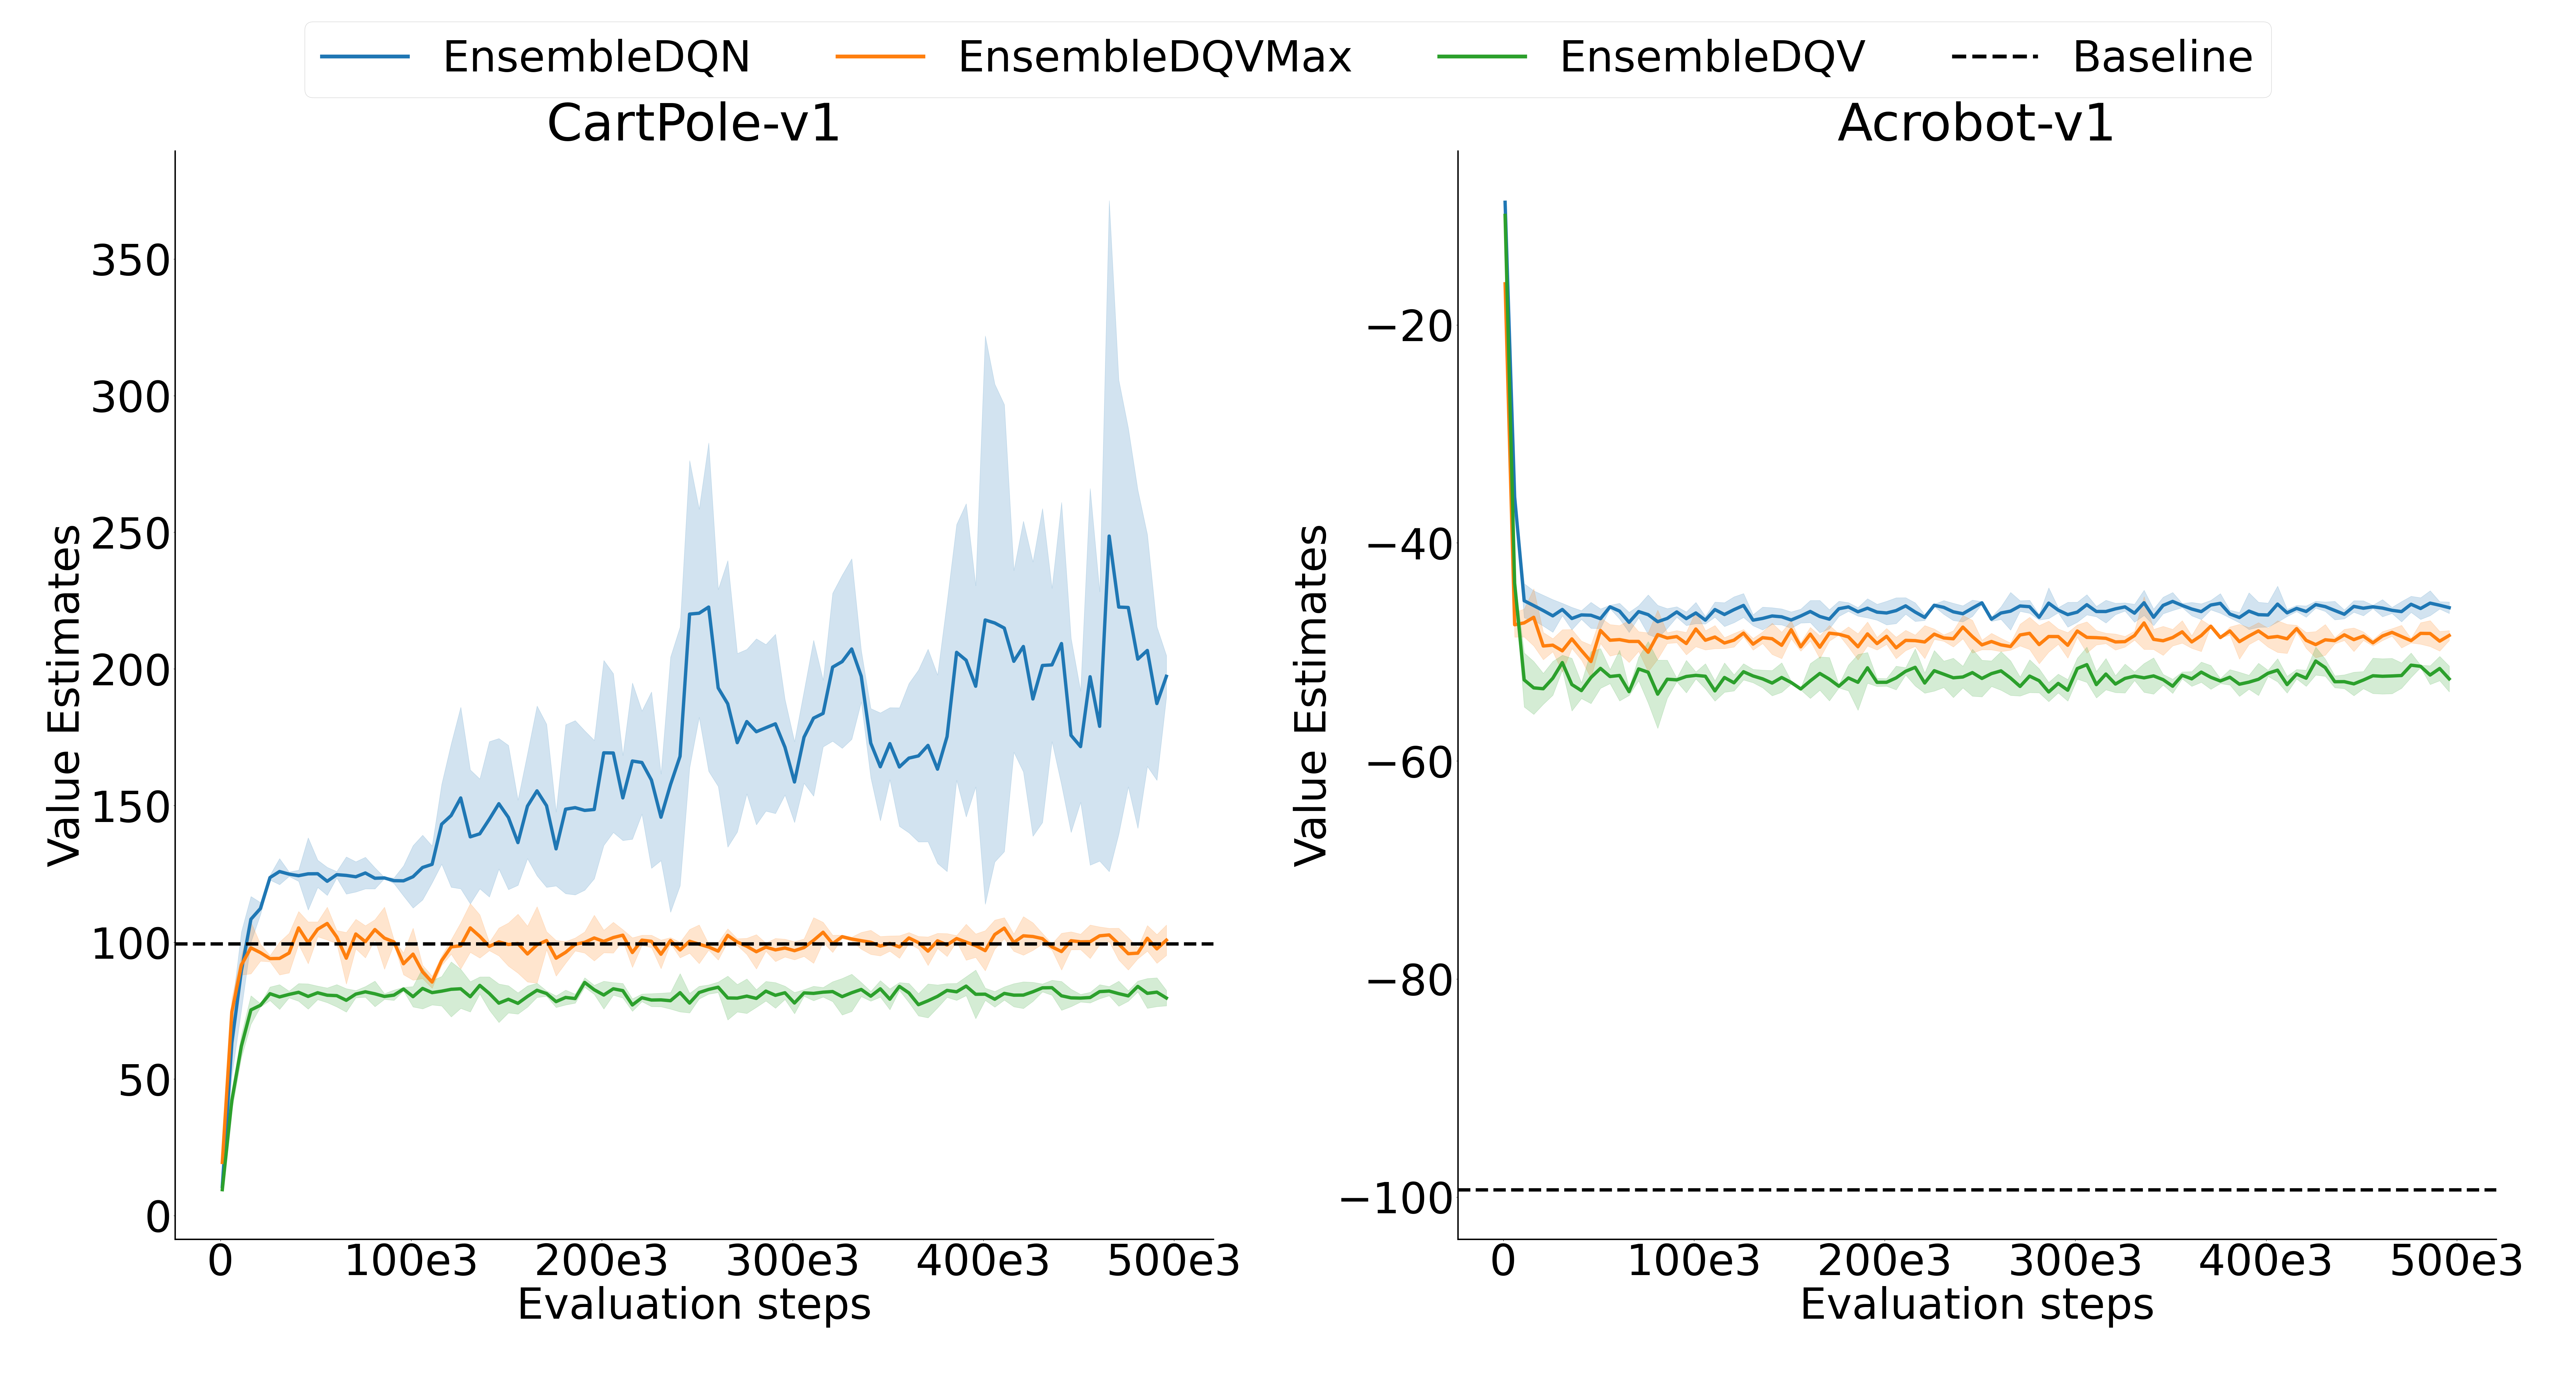
\includegraphics[width=.5\textwidth]{img/dshift_plots_ensembles_qv.png}
  \caption{Evaluation time $Q$-value estimates of the ensemble version
    of offline DQN, DQV and DQV-Max. The shaded areas are $\pm 1$
    standard deviation from the mean of 3 different
    simulations.}\label{fig:dshift_offline_ensemble}
\end{figure}
% TS: ensemble-dqn less optimistically biased, in line with baseline
% results from REM and with theoretical analysis of Averaged-DQN
On the \texttt{CartPole-v1} environment, Offline Ensemble-DQN suffers
from a milder overestimation bias than offline DQN.\ The $Q$-value
estimates on this problem decreased significantly with the
implementation of the ensemble strategy ($t=7.40,p<.01$); moreover, in
line with the theoretical analysis of \citet{anschel2017averaged}, the
observed decrease in $Q$ estimates variance was proportional to the
ensemble number of heads $K$ (8755.07 vs. 2330.90 for Ensemble-DQN and
DQN, respectively). The $Q$-value for $s_0$ still diverges from the
true baseline, as seen in Figure~\ref{fig:dshift_offline_ensemble};
this is a symptomatic that simply ensembling the $Q$ function alone
does not prevent the DQN bootstrapping error. Since the behavior
policy $\pi_{\textrm{DQN}}$ produced a noisy reward signal on the
\texttt{CartPole-v1} environment, the lower $Q$ estimates compared to
base DQN are actually desirable and better capture the ensemble's
uncertainty about the true value of $s_0$. This naturally results in a
significant drop in performance for Ensemble-DQN ($t=2.62,p<.01$),
showing that the agent uses the $Q$-values as a proxy for predicted
reward; full results can be found in Table~\ref{}. Again, the $Q$
estimates on the \texttt{Acrobot-v1} environment for Ensemble-DQN are
stable and overoptimistic, but they do not significantly differ from
those of base offline DQN.\

% TS: Ensemble-DQV and Ensemble-DQVMax no significant changes (reason:
% decoupling, will be addressed again in the Discussion)
Concerning the offline ensemble versions of DQV and DQV-Max, no
significant change in value estimates from their standard counterparts
were observed on both environments. The $Q$-values for these agents in
Figure~\ref{fig:dshift_offline_ensemble} appear very similar to the
non-ensemble variants in Figure~\ref{fig:dshift_offline_normal}. One
notable exception is the performance of offline Ensemble-DQV on the
\texttt{CartPole-v1} environment, where a significant drop was
registered ($t=2.40,p<.01$). However, the $Q$ estimates distributions
for $s_0$ between this agent and offline DQV almost perfectly
overlap (Figure~\ref{fig:qv_dist}). Both offline
DQV and Ensemble-DQV converge to basically the same $Q$-value for
$s_0$, and both cannot incur in an overestimation bias since they only
use the $V$ function to compute the TD-target. Therefore, one
plausible reason for this performance drop is the combination of DQV's
``on-policyness'' with the ensemble technique. Theoretically,
on-policy algorithms should not be able to learn from off-policy data,
yet offline DQV is still able to solve the problems correctly due to
their relative ease. However, it is likely that the incorrect
estimations derived from being on-policy compound together from each
head of the ensemble, producing a sub-optimal policy. To this regard,
it should be noted that the reward accumulated by Ensemble-DQV is
lower than that of base DQV mostly in the early stages of learning
(first 50000 steps) across each run, subsequently stabilizing at the
maximum for the \texttt{CartPole-v1} environment.

%% REVIEW should I introduce this section in the methods first??
%% TODO check the sentence with 'based on the assumption': it is
%% underlying the whole RQ and paper, but is it consistent with previous
%% formulations of the problem?
\subsection{Additional study: Ensemble-DQV-Max ablations}
Since no change was found when using ensembles to estimate both $Q$
and $V$ in DQV-Max, two additional experiments were performed where
either the $Q$ or the $V$ function were approximated by an ensemble,
respectively. This further investigation is motivated by the fact
that, like DQN, DQV-Max is an off-policy algorithm, hence of interest
for offline RL.\ Moreover, since DQV-Max already decouples selection
and evaluation, we want to assess whether either value function
involved in the computation of DQV-Max's TD-targets drives more
bootstrapping error than the other, based on the assumption that
ensemble techniques should dampen $Q$-values.
\begin{figure}[!tbp]
  \centering
  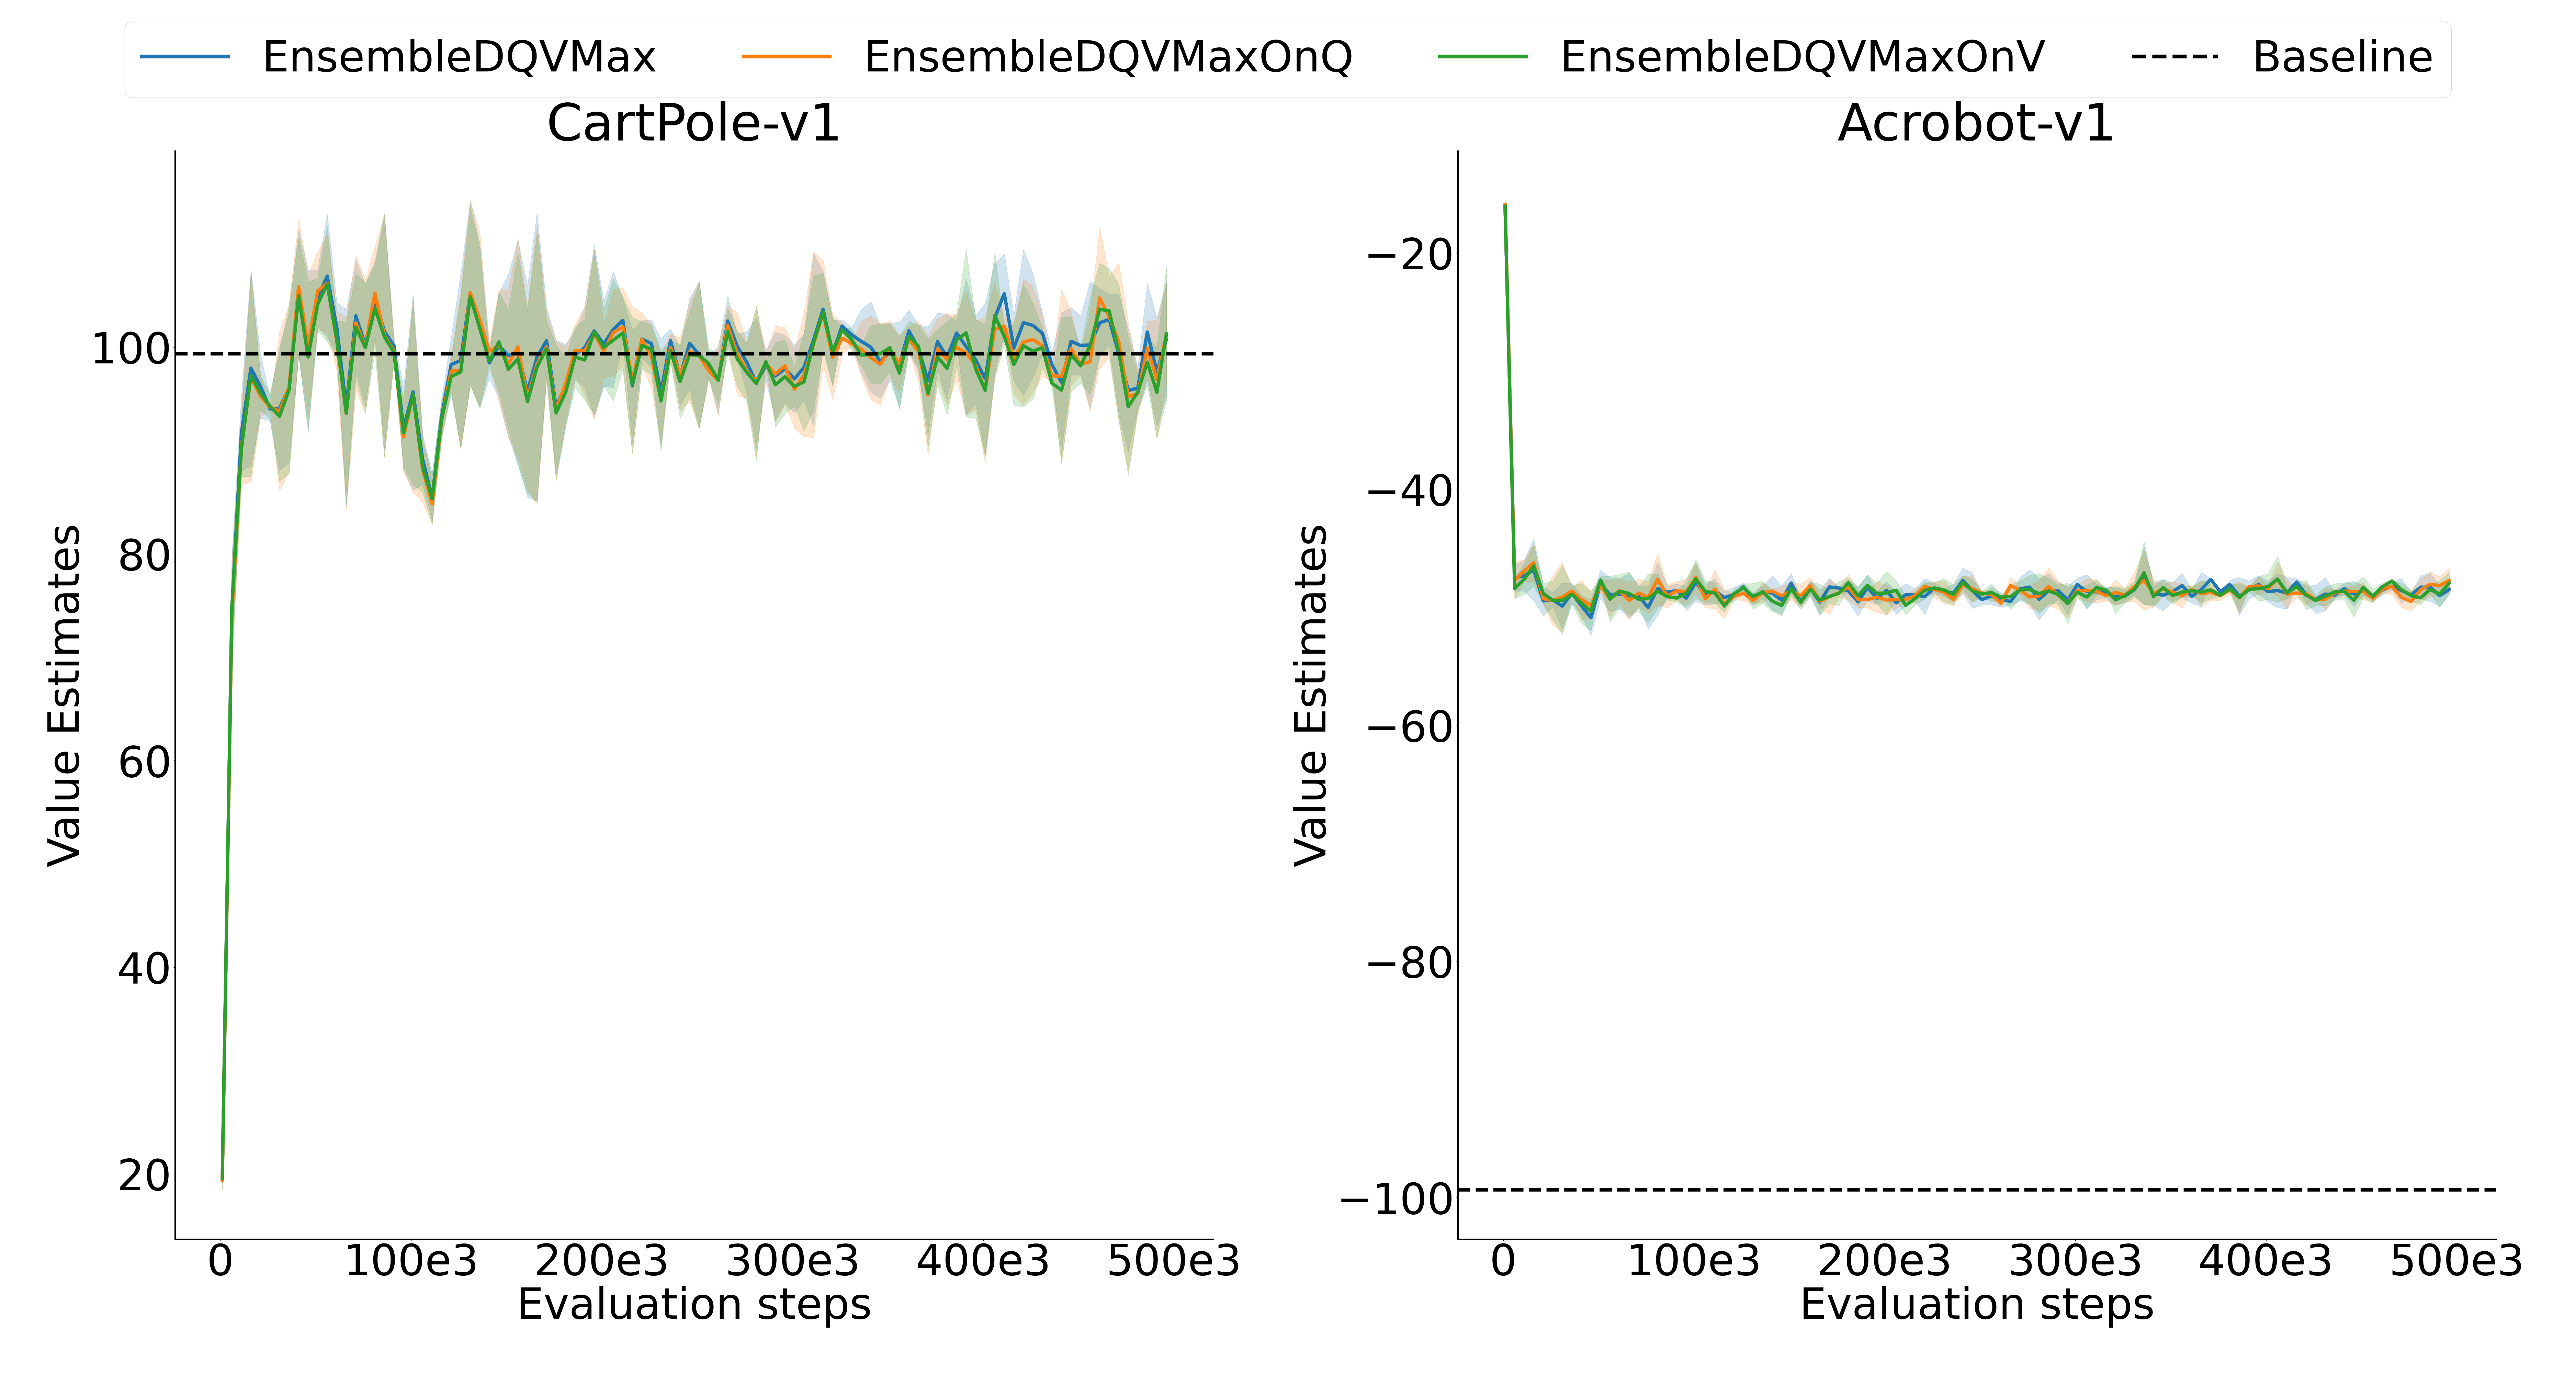
\includegraphics[width=.5\textwidth]{img/dshift_plots_ablation_qv.png}
  \caption{Evaluation time $Q$-value estimates of the ablated variants
    of offline Ensemble-DQV-Max. The shaded areas are $\pm 1$ standard
    deviation from the mean of 3 different
    simulations.}\label{fig:dshift_dqvmax_ablations}
\end{figure}
As seen in Figure~\ref{fig:dshift_dqvmax_ablations}, results for these
experiments are clear: ensembling either only the $Q$ function
(EnsembleDQVMaxOnQ) or the $V$ function (EnsembleDQVMaxOnV) results in
fundamentally the same $Q$ estimates for $s_0$ as produced by
ensembling both functions. Looking at the DQV-Max temporal difference
targets for $V$ and $Q$ (Equation~\ref{dqvmax:v_td_target}
and~\ref{dqvmax:q_td_target}, respectively) the reason is evident: the
$Q$ function regresses towards targets computed by $V$, which cannot
suffer from the action distributional shift, thus updates to $Q$ are
in-distribution with respect to the training data. Ultimately, this is
probably enough to correct bootstrapping errors arising when computing
the targets for $V$, and the two value functions are able to balance
their respective estimates, such that using an ensemble on either
results in no significant change.

%% TODO appendix:
%% - table with mean and variance (or std) for each agent on each
%%   environment, coloring entries that show significant differences
%% - hyper-parameters
